\documentclass[12pt]{beamer}
\author{Yan Wang}
\title{Paper reading seminar}
\subtitle{}
\usetheme{Malmoe}
\setbeamertemplate{navigation symbols}{}
\newcommand*\oldmacro{}%
\let\oldmacro\insertshorttitle%
\renewcommand*\insertshorttitle{%
\oldmacro\hfill%
\insertframenumber\,/\,\inserttotalframenumber}

\begin{document}

\begin{frame}[plain]
	\titlepage
\end{frame}

\begin{frame}{What Has My Classifier Learned? Visualizing the Classification Rules of Bag-of-Feature Model by Support Region Detection}
    \begin{itemize}
        \item Interesting
        \begin{itemize}
            \item Motivation
            \item Applications
        \end{itemize}
        \item Motivation
        \begin{itemize}
            \item Critical parts of the image for classification
            \item Sparse Coding + Max Polling
        \end{itemize}
    \end{itemize}
\end{frame}

\begin{frame}{Background}
    \begin{itemize}
        \item Related work: heat map (Li Fei-Fei, CVPR 11)
        \begin{itemize}
            \item SVM + random forest + dense sampling $\Rightarrow$ image classification
            \item Image region selection $\Rightarrow$ heatmap
            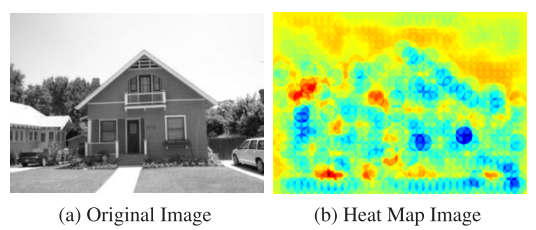
\includegraphics[width=0.6\textwidth]{fig1.png}
        \end{itemize}
        \item Assumption
        \begin{itemize}
            \item SC + MP $\Rightarrow$ no linearity: $C(A \cup B) \neq \mu C(A) + (1 - \mu) C(B)$
            \item Interested in regions without which the image will be misclassified
        \end{itemize}
    \end{itemize}
\end{frame}

\begin{frame}{Approach}
    \begin{itemize}
        \item SC + MP
        \begin{itemize}
            \item Sparse coding: $u_j \in \mathbb{R}^V$. $u_{jk}$
            \item Pooling: $\max_j \{u_{jk}\}$
            \item Classification: $\hat{y} = \mathop{sgn} \Big( w_k \max_j \{u_{jk}\} + b \Big)$
        \end{itemize}
        \item Support Region $R_s$
        \begin{itemize}
            \item Only interested in positive samples
            \[ \sum_k \max_{\{j|P_j \notin R_s \}} \{ u_{jk} \} + b < 0 \]
            \item Restriction on area
        \end{itemize}
    \end{itemize}
\end{frame}

\begin{frame}{Approach}
    \begin{itemize}
        \item An efficient (DP-like) way to detect such regions
        \[ J(R_p, R_q) = \sum_k w_k \Big( \max_{\{j|P_j\in R_p\}} \{u_{jk}\} - \max_{\{j|P_j\in R_p-R_q\}} \{u_{jk}\} \Big) \]
        \item Don't really know what it means... The larger, the better? $R_q \subset R_p$
        \[ K(I, R_s) \geq S_0, S_0 = \sum_k \max_j \{u_{jk}\} + b \]
        \[ J(I, R_t) = J(I, R_{t - 1} + J(I - R_{t - 1}, P_t) \]
        \item Iteration way. Start from $P_0$, $R_t = R_{t - 1} \cup \hat{P}_t$
        \[ \hat{P}_t  = \arg \max_{P_t \in \text{boundary}\{R_{t-1}\}} J(I - R_{t - 1}, P_t) \]
    \end{itemize}
\end{frame}

\begin{frame}{Applications}
    \begin{itemize}
        \item Predict the failure mode of classifiers
        \medskip
        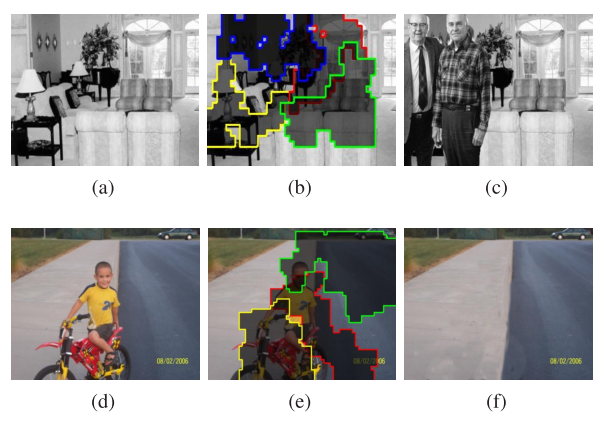
\includegraphics[width=0.6\textwidth]{fig2.png} \\
    \end{itemize}
\end{frame}

\begin{frame}{Applications}
    \begin{itemize}
        \item Understand the classification and discover database bias
        \medskip
        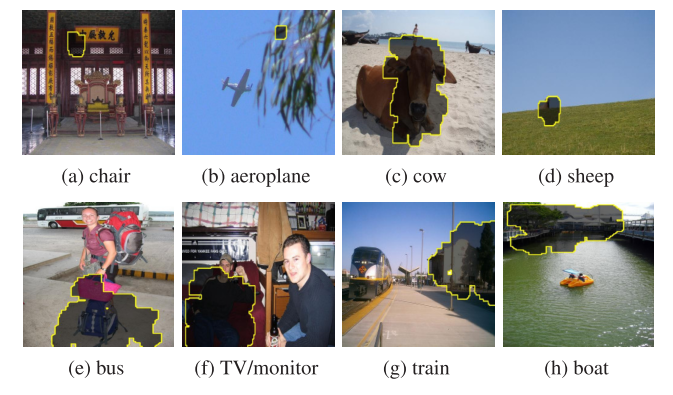
\includegraphics[width=0.6\textwidth]{fig3.png} \\
    \end{itemize}
\end{frame}

\begin{frame}{Applications}
    \begin{itemize}
        \item Understand the classification and discover database bias
        \medskip
        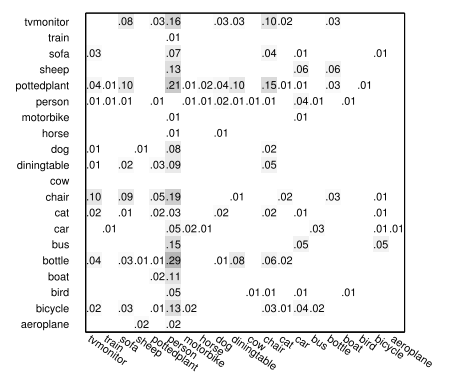
\includegraphics[width=0.6\textwidth]{fig5.png} \\
    \end{itemize}
\end{frame}

\begin{frame}{Applications}
    \begin{itemize}
        \item Build better classifiers
        \begin{itemize}
            \item User annotates bad support regions $\Rightarrow$ remove the regions, put remaining image as a positive sample
            \item Cross-dataset validation: context won't help, must focus on the objects themselves
        \end{itemize}
        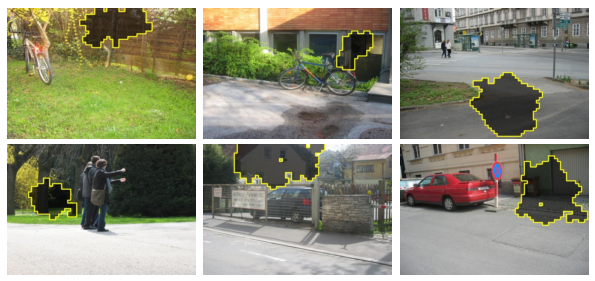
\includegraphics[width=0.6\textwidth]{fig6.png} \\
    \end{itemize}
\end{frame}

\begin{frame}{Applications}
    \begin{itemize}
        \item Build better classifiers
        \begin{itemize}
            \item User annotates bad support regions $\Rightarrow$ remove the regions, put remaining image as a positive sample
            \item Cross-dataset validation: context won't help, must focus on the objects themselves
        \end{itemize}
        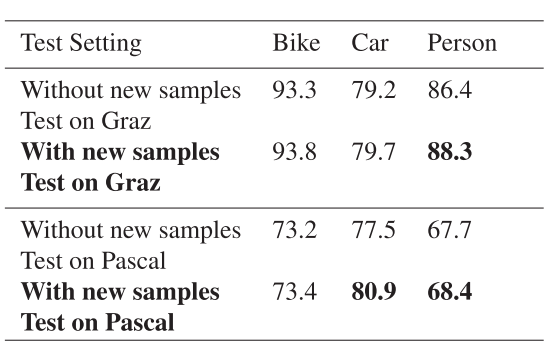
\includegraphics[width=0.6\textwidth]{tbl1.png} \\
    \end{itemize}
\end{frame}

\begin{frame}{Ensemble of Exemplar-SVMs for Object Detection and Beyond}
	\begin{itemize}
		\item Motivation
		\begin{itemize}
			\item ``Semantic classifier'' hard because things are not visually similar
			\item Build ``exemplar classifier'' to do instance classification and then fuse the scores
			\item SVM-style extension of KNN-based classification
		\end{itemize}
		\item New problem
		\begin{itemize}
			\item Detection dataset $\Rightarrow$ matching instance $\Rightarrow$ associated metadata (class, label, 3D model, segmentation, ...)
		\end{itemize}
	\end{itemize}
\end{frame}

\begin{frame}{Approach}
	\begin{itemize}
		\item Exemplar-SVM
		\begin{itemize}
			\item Corresponds to every (detection) instance
			\item Positive training sample: detection instance
			\item Negative training sample: all the other instances
			\item HoG + Linear SVM
			\item Use non-maximum suppression in testing phrase
		\end{itemize}
	\end{itemize}
\end{frame}

\begin{frame}{Approach}
	\begin{itemize}
		\item Calibration
		\begin{itemize}
			\item The individually trained SVMs have different scales
			\item Cannot be integrated for final result directly
			\item Calibration to normalize their score
			\item For every Exemplar-SVM
			\[f(x|w_E,\alpha_E,\beta_E) = \frac{1}{1 + e^{-\alpha_E(W_E^Tx-\beta_E)}}\]
			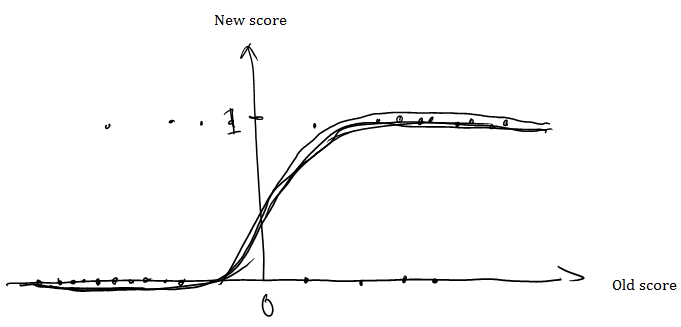
\includegraphics[width=0.8\textwidth]{esvm-calibration.png}
		\end{itemize}
	\end{itemize}
\end{frame}

\begin{frame}{Approach}
	\begin{itemize}
		\item Calibration
		\begin{itemize}
			\item Sample collection
			\begin{itemize}
				\item Agreed samples (w/in one class?) $\Rightarrow$ positive samples
				\item Other samples %\Rightarrow$ negative samples
			\end{itemize}
		\end{itemize}
		\item Test
		\begin{itemize}
			\item Sliding window + HoG
			\item Individual test score
			\item Calibrated test score
			\item Sum?
		\end{itemize}
	\end{itemize}
\end{frame}

\begin{frame}{Data-driven Visual Similarity for Cross-domain Image Matching}
	\begin{itemize}
		\item Problem: cross-domain image matching
		\item Motivation
		\begin{itemize}
			\item Visual similarity metric is hard to design
			\item Directly use the (unlabeled) data
			\item Training a discriminative classifier to discover important parts of an image $\Rightarrow$ learn a similarity metric from data
		\end{itemize}
	\end{itemize}
\end{frame}

\begin{frame}{Approach}
	\begin{itemize}
		\item Train an SVM for every image
		\begin{itemize}
			\item Pos: one image with shifting/rotating/scaling
			\item Neg: (millions of) sliding windows from (10K) randomly sampled Flickr images
			\item Feature: grid-like features with high enough dimensions, like HoG or Dense SIFT
		\end{itemize}
		\item Technical details
		\begin{itemize}
			\item Efficiency: SVM only keeps support vectors in the negative part $\Rightarrow$ efficient in testing phrase
			\item ``Sample expansion'': explore more negative samples with current trained $w$
			\item Ranking: didn't find in the paper
		\end{itemize}
	\end{itemize}
\end{frame}

\begin{frame}{Experiments}
	\begin{itemize}
		\item Perform well in saliency detection
		\item Image-Image matching
		\begin{itemize}
			\item Dataset: INRIA Holiday Dataset to ensure the exact query instance exists in the dataset
			\item Baselines: GIST, Tiny images, spatial pyramid
			\item Measurement: true positive rate in top 100 results
		\end{itemize}
	\end{itemize}
\end{frame}

\begin{frame}{Experiments}
	\begin{itemize}
		\item Sketch-Image matching
		\begin{itemize}
			\item Dataset: 25 car sketch + 25 bike sketch against PASCAL VOC 2007 and SBIR Dataset
			\item Baselines: proposed algo. with different dataset size
			\item Measurement: mAP of top K
		\end{itemize}
		\item Point-Image matching (qualitative)
		\begin{itemize}
			\item Dataset: self-collected, 50 outdoor paintings agains 5K GPS-enabled images within 50 miles and 5K random images
		\end{itemize}
	\end{itemize}
\end{frame}

\begin{frame}{Applications}
	\begin{itemize}
		\item Scene completion
		\item Internet re-photography
		\item Painting2GPS
		\item Visual Scene Exploration
	\end{itemize}
\end{frame}

\end{document}
